\documentclass[xelatex,ja=standard,jafont=noto]{bxjsarticle}
\usepackage[utf8]{inputenc}

\date{JUNE 2020}

\usepackage{natbib}
\usepackage{graphicx}
\usepackage{tikz}
\usepackage{circuitikz}
\usepackage{tabularx}
\usepackage{diagbox}
\usepackage{amsmath,amssymb}
\usepackage{hyperref}


\begin{document}


	\begin{titlepage}
			\begin{center}
				
				{\Large 令和2年}
				
				\vspace{10truept}
				
				{\Large 機械工学実験1}
				
				\vspace*{140truept}
				
				{\Huge 振動実験プリレポート} 
				
				\vspace{160truept}
				
				{\Large 指導教員}
				
				\vspace{10truept}
				
				{\Large Toshio Itou}
				
				\vspace{70truept}
				
				{\Large 芝浦工業大学}
				
				\vspace{10truept}
				
				{\Large 機械制御システム}
				
				\vspace{30truept}
				
				{\Large bq18026 関宇}      
				
			\end{center}
		\end{titlepage}

\section{課題1}

固有振動数の物理的な意味を説明せよ.また,機械設計において固有振動数を知ることが重要である理由を説明せよ.\\

固有振動数というのは振動系自身の性質によって特有の振動のことである.機械設計する時に事故を防ぐことも重要となってくる.しかし加振力が固有振動数とともに振動する時に共振という現象が発生し,振幅が大きくなって事故が起こしやすいので,これを防ぐために固有振動数を知ることが重要である.$ ^{[1]} $



\section{課題2}

実験で使用するはりの材料はSUS405とSS400の2種類である.それぞれについて,縦弾性係数と密度を調べよ.必ず出典を明記すること.$ ^{[6][7]} $


\begin{table}[!htbp]
\centering
\caption{<金属材料データベース>}
\begin{tabular}{ccc}
\hline
& SUS405 & SS400 \\
\hline
縦弾性係数(KN/mm^{2})& 200& 205\\
密度(kg/m^{3}) & 7750& 7850\\
\hline
\end{tabular}
\end{table}



\section{課題3}

図 1 のような幅 b,厚さ h の一様な長方形断面のはりの中立軸 N-N'まわりの断面二次モーメント I を
b と h を用いて表せ.また,断面 2 次モーメントの物理的な意味を説明せよ.$ ^{[4]} $


\begin{figure}[h!]
    \centering
    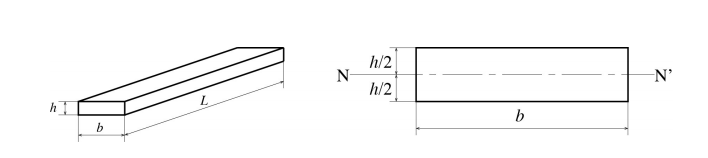
\includegraphics[scale=0.6]{control/振动/01.png}
    \caption{はりの断面形状}
\end{figure}


まず,断面二次モーメントIは定義である(1)式は以下である.


\begin{equation}
			I=\int_{A}^{}y^{2}dA
\end{equation}


ここで,微小面積dAは微小長さdyを用いると,$ dA=bdy $と表せる.さらに積分範囲は中立軸まわりだから,$ -\frac{h}{2}\sim\frac{h}{2} $.これより

\begin{equation}
			I=\int_{-\frac{h}{2}}^{\frac{h}{2}}y^{2}bdy=\frac{bh^{3}}{12}
\end{equation}


\section{課題4}
(4) 図 2 のように片持ちばりの先端に鉛直下方に力 F を加えたところ,先端にの変位が生じた.F との
関係を次式のように表したときの k が片持ちばりをばねとみなしたときのばね定数(等価ばね定数)
である.$ ^{[5]} $



\begin{equation}
			F=k\delta
\end{equation}

ばね定数 k を縦弾性係数 E,断面二次モーメント I,はりの長さ L を用いて表せ.



\begin{figure}[h!]
    \centering
    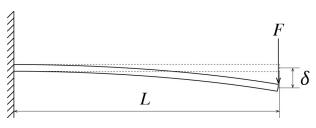
\includegraphics[scale=0.6]{control/振动/02.png}
    \caption{先端に力が作用する片持ちばり}
\end{figure}


まず先端からの距離Lにおける曲げモーメントM=-FL,これをはりのたわみ方程式に代入して2回微分すればたわみ曲線の方程式が出る.


\begin{equation}
		\frac{d^{2}\delta}{dx^{2}}=-\frac{M}{EI}=\frac{Fx}{EI}
\end{equation}

1回目

\begin{equation}
		\frac{d\delta}{dx}=\int\frac{Fx}{EI}dx=\frac{F}{2EI}x^{2}+C_{1}
\end{equation}

続いて2回目の積分


\begin{equation}
		\delta=\int(\frac{F}{2EI}x^{2}+C_{1})dx=\frac{F}{6EI}+C_{1}x+C_{2}
\end{equation}

これを求めるには積分定数の$ C_{1},C_{2} $を境界条件から決める.また,最大たわみははりの先端,すなわちx=0で生じるから,

\begin{equation}
	\delta=\frac{FL^{3}}{3EI}
\end{equation}


$ F=k\delta $から,$ k=\frac{F}{\delta} $.よって,



\begin{equation}
	k=\frac{3EI}{L^{3}}
\end{equation}



\newpage


\section{課題5}
はりの横振動の運動方程式を導出せよ.$ ^{[2]} $

\begin{equation}
			\frac{\partial^{2}}{\partial x^{2}}[EI\frac{\partial^{2}y}{\partial x^{2}}]+\rho A\frac{\partial^{2}y}{\partial t^{2}}=0
\end{equation}


\begin{figure}[h!]
    \centering
    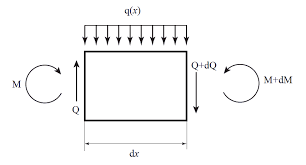
\includegraphics[scale=0.6]{control/振动/03.png}
    \caption{はりの微小要素}
\end{figure}



ニュートンの方程式F=maより,微小要素y方向の運動方程式は,

\begin{equation}
			(\rho Adx)\frac{\partial^{2}y(x,t)}{\partial t^{2}}=Q+\frac{\partial Q}{\partial x}dx-Q=\frac{\partial Q}{\partial x}dx
\end{equation}

となる.そしてせん断力Q(x,t)をたわみy(x,t)であらわすため,まず座標x+dxの位置に関するモーメントのつり合いを考えると,


\begin{equation}
			M(x,t)+\frac{\partial M(x,t)}{\partial x}dx-M(x,t)+Q(x,t)dx=0
\end{equation}

となり,次式を得る.


\begin{equation}
			\frac{\partial M(x,t)}{\partial x}d=-Q(x,t)
\end{equation}


材料力学の知識より,曲げモーメントとそれによって生じる変位との関係は次式で与えられる.


\begin{equation}
			EI(x)\frac{{\partial^{2}y(x,t)}}{\partial x^{2}}=M(x,t)
\end{equation}


式を代入すると次式を得る


\begin{equation}
			\rho A(x)\frac{\partial^{2}y(x,t)}{\partial t^{2}}+\frac{\partial^{2}}{\partial x^{2}} (EI(x)\frac{\partial^{2}y(x,t)}{\partial x^{2}})=0
\end{equation}


これがはりの運動方程式である.とくに,はりが均質で一様な断面を持つ場合は,$ EI(x),A(x) $は一定であるので,上式は以下のようになる.


\begin{equation}
			\rho A\frac{\partial^{2}y(x,t)}{\partial t^{2}}+EI\frac{\partial^{4}y(x,t)}{\partial x^{4}}=0
\end{equation}


\newpage



\section{課題6}
片持ちばりの横振動の境界条件として自由端において次の関係を与える.$ ^{[3]} $



\begin{equation}
			\frac{\partial^{2}y}{\partial x^{2}}=0, \frac{\partial^{3}y}{\partial x^{3}}=0
\end{equation}\\


自由端の境界条件がこのように表される理由を説明せよ.\\


境界条件としては,自由端の曲げモーメントは0である.式より,$ \frac{\partial^{2}y}{\partial x^{2}}=0 $である.\\

そしてせん断力も0である.$ \frac{\partial M(x,t)}{\partial x}d=-Q(x,t) $より,せん断力$ Q(x,t)=-EI(x)\frac{\partial^{3}y}{\partial x^{3}} $,つまり$ \frac{\partial^{3}y}{\partial x^{3}}=0 $である.



\newpage


\section{}
\begin{thebibliography}{9}
\bibitem{latexcompanion} 
岩壺 卓三,松久 寛, 井上喜雄, 宇津野秀夫, 河村庄造, 神吉博, 小泉孝之, 塩幡宏規  
[\textit{振動工学の基礎}]. 
森北出版株式会社,  2019/2/20,  第一章:機械の振動 振動事故例 p5

\bibitem{latexcompanion} 
岩壺 卓三,松久 寛, 井上喜雄, 宇津野秀夫, 河村庄造, 神吉博, 小泉孝之, 塩幡宏規  
[\textit{振動工学の基礎}]. 
森北出版株式会社,  2019/2/20,  第5章:連続体の振動 はりの振動 p116-117

\bibitem{latexcompanion} 
岩壺 卓三,松久 寛, 井上喜雄, 宇津野秀夫, 河村庄造, 神吉博, 小泉孝之, 塩幡宏規  
[\textit{振動工学の基礎}]. 
森北出版株式会社,  2019/2/20,  第5章:連続体の振動 はりの振動 p118



\bibitem{latexcompanion} 
沢 俊行 
[\textit{再入門・材料力学 基礎編}]. 
ものづくりの教科書,  2007/10/22,  第5章:断面二次モーメントと断面係数  p107



\bibitem{latexcompanion} 
沢 俊行 
[\textit{再入門・材料力学 基礎編}]. 
ものづくりの教科書,  2007/10/22,  第6章:曲げモーメントを受けるはりのたわみ方  p133





\bibitem{einstein} 
ステンレス協会
[\textit{ステンレスのヤング率、ポアソン比など機械的性質について}]. 
\url{http://www.jssa.gr.jp/contents/faq-article/q6/}


\bibitem{einstein} 
ステンレス協会
[\textit{主な機械材料の物理的性質}]. 
\url{http://www.me.cit.nihon-u.ac.jp/lab/ben/LectureCourse/New_1Mechanics/Material_Properties.pdf}



\end{thebibliography}





\end{document}